\documentclass[]{book}

%These tell TeX which packages to use.
\usepackage{array,epsfig}
\usepackage{amsmath}
\usepackage{amsfonts}
\usepackage{amssymb}
\usepackage{amsxtra}
\usepackage{amsthm}
\usepackage{mathrsfs}
\usepackage{color}
\usepackage[margin=2cm,top=2.5cm,headheight=16pt,headsep=0.1in,heightrounded]{geometry}
\usepackage{fancyhdr}
\pagestyle{fancy}
\usepackage{pgfplots}

\pgfplotsset{compat = newest}

%Here I define some theorem styles and shortcut commands for symbols I use often
\theoremstyle{definition}
\newtheorem{defn}{Definition}
\newtheorem{thm}{Theorem}
\newtheorem{cor}{Corollary}
\newtheorem*{rmk}{Remark}
\newtheorem{lem}{Lemma}
\newtheorem*{joke}{Joke}
\newtheorem{ex}{Example}
\newtheorem*{soln}{Solution}
\newtheorem{prop}{Proposition}

\newcommand{\lra}{\longrightarrow}
\newcommand{\ra}{\rightarrow}
\newcommand{\surj}{\twoheadrightarrow}
\newcommand{\graph}{\mathrm{graph}}
\newcommand{\bb}[1]{\mathbb{#1}}
\newcommand{\Z}{\bb{Z}}
\newcommand{\Q}{\bb{Q}}
\newcommand{\R}{\bb{R}}
\newcommand{\C}{\bb{C}}
\newcommand{\N}{\bb{N}}
\newcommand{\M}{\mathbf{M}}
\newcommand{\m}{\mathbf{m}}
\newcommand{\MM}{\mathscr{M}}
\newcommand{\HH}{\mathscr{H}}
\newcommand{\Om}{\Omega}
\newcommand{\Ho}{\in\HH(\Om)}
\newcommand{\bd}{\partial}
\newcommand{\del}{\partial}
\newcommand{\bardel}{\overline\partial}
\newcommand{\textdf}[1]{\textbf{\textsf{#1}}\index{#1}}
\newcommand{\img}{\mathrm{img}}
\newcommand{\ip}[2]{\left\langle{#1},{#2}\right\rangle}
\newcommand{\inter}[1]{\mathrm{int}{#1}}
\newcommand{\exter}[1]{\mathrm{ext}{#1}}
\newcommand{\cl}[1]{\mathrm{cl}{#1}}
\newcommand{\ds}{\displaystyle}
\newcommand{\vol}{\mathrm{vol}}
\newcommand{\cnt}{\mathrm{ct}}
\newcommand{\osc}{\mathrm{osc}}
\newcommand{\LL}{\mathbf{L}}
\newcommand{\UU}{\mathbf{U}}
\newcommand{\support}{\mathrm{support}}
\newcommand{\AND}{\;\wedge\;}
\newcommand{\OR}{\;\vee\;} 
\newcommand{\Oset}{\varnothing}
\newcommand{\st}{\ni}
\newcommand{\wh}{\widehat}
\newcommand{\vect}[1]{\overrightarrow{#1}}

%Pagination stuff.
\setlength{\topmargin}{-.3 in}
%\setlength{\oddsidemargin}{0in}
%\setlength{\evensidemargin}{0in}
\setlength{\textheight}{9.in}
\setlength{\textwidth}{6.5in}
\cfoot{page \thepage}
\lhead{MEU301 - Analyse}
\rhead{TD1}
\pagestyle{fancy}


\begin{document}

\subsection*{Rappel de cours}

\newpage

\subsection*{Exercice 1}

$$
f_n(x) = 1/n 1_{[0, n]} = 
\left\{
\begin{array}{l l}
1/n & x \in [0,n] \\
0 & sinon
\end{array}
\right.
$$

Pour un $x$ donn\'e, prenons $\epsilon > 0$ et un $n_0$ arbitraire, pour tout $n > n_0$, on a $f_n(x) > f_{n_0}(x)$ sur la partie $x \in [n_0, n]$ car par d\'efinition $f_{n_0}(x) = 0$ pour $x > n_0$. Donc pour chaque $\epsilon$ on peut trouver un $n$ tel que $f_n(x) > \epsilon$, la fonction ne converge pas simplement.


\subsection*{Exercice 2}


$$
f_n(x) = n 1_{[0, 1/n]} = 
\left\{
\begin{array}{l l}
n & x \in [0,1/n] \\
0 & sinon
\end{array}
\right.
$$

Pour un $x$ donn\'e, prenons $\epsilon > 0$ et un $n_0$ tel que $n_0 > 1/\epsilon$. Pour tout $n > n_0$ on a $f_n(x) < \epsilon$ car sur $[0,1/n]$ $f_n(x) = f_{n_0}(x)$ et sur $[1/n,1/n_0]$ on a $f_n(x) = 0$. 	 
Donc la fonction converge simplement.

\subsection*{Exercice 3}

\begin{tikzpicture}[scale=1.0]
\begin{axis}[
    xmin = -7, xmax = 7,
    ymin = -0.5, ymax = 2.0]
    \addplot[
        domain = -5:5,
        samples = 200,
        smooth,
        thick,
        blue,
    ] {1/(1+x^2+x^4};
    \addplot[
        domain = -5:5,
        samples = 200,
        smooth,
        thick,
        yellow,
    ] {1/(1+10*x^2+x^4};
    \addplot[
        domain = -5:5,
        samples = 200,
        smooth,
        thick,
        red,
    ] {1/(1+50*x^2+x^4};
\end{axis}
\end{tikzpicture}


Convergence simple. Pour un x donn´e, prenons $\epsilon> 0$ et $n_0$ tel que $\frac{1}{1+n_0x^2+x^4)} < \epsilon$ donc $n_0 > \frac{1/\epsilon-1-x^4}{x^2}$. Dans ce cas, $\forall n \geq n_0, f_n(x) < \epsilon$ donc la s´erie de fonction converge simplement. $\lim_{n \to \infty}{f_n(x)} = 0$ donc $f_n(x)$ tend vers 0.


Convergence uniforme. Calculons $\sup(\lim_{n \to \infty} {|f_x(x) - 0||}) =  \sup(\lim_{n \to \infty} {f_n(x)}) = 1$ lorsque $x=0$. Donc la s\'erie ne converge pas uniform\'ement.

Prenons $g_n(x) = \frac{1}{1+nx^2}$ on a $\forall x, n, f_n(x) < g_n(x)$. Donc si la fonction $g_n(x)$ converge uniform\'ement alors $f_n(x)$ converge \'egalement. Calculons $\int{\frac{1}{1+nx^2} dx}$ avec $u = \sqrt{n}x$, donc $\frac{du}{dx} = \sqrt{n}$ et $dx= \frac{1}{\sqrt{n}} du$
$$
\int{\frac{1}{1+nx^2} dx} = \int{\frac{1}{1+u^2} \frac{1}{\sqrt{n}} du} = \frac{1}{\sqrt{n}} \int{\frac{1}{1+u^2} du} = \frac{1}{\sqrt{n}} \arctan(u) = \frac{\arctan(\sqrt{n}x)}{\sqrt{n}} 
$$

On a $\forall x, n \sup(\arctan(\sqrt{n}x))) = \frac{\pi}{2}$ donc $\lim_{n \to n} \forall x \sup(g_n(x)) = 0$. Donc l'int\'egrale de $g_n(x)$ converge uniform\'ement et par cons\'equent l'int\'egrale de $f_n(x)$ converge \'egalement uniform\'ement.



\end{document}

